\documentclass{report}
\usepackage[utf8]{inputenc}
\usepackage[T1]{fontenc} 
\usepackage[francais]{babel}
\usepackage{colortbl}
\usepackage{amssymb}
\usepackage{pgf, tikz}
\usepackage{xcolor}
\usepackage{array}
    \title{\textit{Rapport} \\ La compression}
    \author{Lucas \textsc{Labadens} \and Isabelle \textsc{Marino} }
    \date{Le \today}
\begin{document}
\maketitle
 

\section*{Introduction}
La compression de données ou codage de source est un processus informatique permettant de transformer un document sous forme binaire en un autre document contenant une suite de bit plus courte que le précédent mais pouvant restituer les mêmes informations en utilisant un algorithme de décompression propre à la méthode de compression  utilisé. En d'autres termes, la compression raccourcit la taille des données. La décompression est l'opération inverse de la compression.

Il y a notamment 2 grands types de compression:
\begin{itemize}
\item la compression sans perte de données
\item la compression avec perte de données
\end{itemize}

Un algorithme de compression sans perte restitue après compression et décompression un document strictement identique à l'original. Les algorithmes de compression sans perte sont utiles pour les documents, les archives, les fichiers exécutables ou les fichiers textes.
Pour la compression de données sans perte, on distingue principalement deux types de codage : le codage entropique et le codage algorithmique.

Avec un algorithme de compression avec perte, la suite de bits obtenue après  compression,  est différente de l'originale, mais l'information restituée est très proche. Les algorithmes de compression avec perte sont utiles pour les images, le son et la vidéo.

Les formats de données tels que ZIP, BZIP2, XZ, GZIP, MP3 et JPEG utilisent des algorithmes de compression de données.
La compression est un procédé très utilisé dans la vie courante pour, par exemple, envoyer certains documents par e-mails ou pour le skockage de documents sur disque dur ou cloud center.
  
Le but de notre projet est de compresser des fichiers sans perte de données. 
Nous allons donc vous présenter différents algorithmes de compression sans perte de données que nous avons codés puis testés.

Dans un premier temps nous vous présenterons le codage de Huffman statique et celui de Lempel-Ziv. 
Pour cela nous avons choisit d'utiliser le langage Java pour nous permettre d'avoir des classes structurées et codées les différents algorithmes tout en gardant une structure et des fonctions communes.
 \part*{Algorithme de compression}
\chapter*{Huffman statique}
\section*{Définition et Exemple }
\subsubsection*{Définition}
Dans chaque langue on peut remarquer que certain caractères apparaissent plus que d'autre et cela est valable pour n'importe quel langage informatique. L'algorithme de Huffman utilise cette redondance de caractère pour compresser un fichier.  Un caractère est codé sur un octet quelque soit sa fréquence d'apparition, l'algorithme d'Huffman va donc codé chaque caractère sur un nombre de bit différent en faisant en sorte que les caractères les plus redondants soit codés sur le moins de bit possible. L'algorithme d'Huffman est un codage entropique car celui-ci nécessite de laisser des informations sur l'arbre de compression, dans le fichier compressé, qui seront utilisées lors de la décompression.
\subsection*{Compression}
La compression est décomposé en plusieurs parties:
\begin{itemize}
\item[-] Une première partie, qui consiste à lire une première fois le fichier que l'on veut compresser et à compter le nombre d'apparition de chaque caractère. On considère ensuite que chaque caractère à un poids qui correspond à son nombre d'apparition. On va ensuite procéder à la construction d'un arbre binaire de compression. Un arbre de compression est composé de poids, qui se divise en deux types : les feuilles composées d'un caractère et d'un poids et les  nœuds composés d'un fils gauche et droit et d'un poids. Pour créer notre arbre, on trie les feuilles, obtenues lors de la première lecture, par ordre croissant de poids. Puis on relie les deux feuilles de poids plus faibles par un nœud de poids égal à la somme du poids des deux feuilles reliées.  Ensuite, on enlève les deux feuilles reliées de la liste, on ajoute le nouveau le  nœud à  la liste et on la trie à nouveau. On répète l'opération jusqu'à qu'il ne reste plus qu'un seul poids, ce sera la racine de notre arbre binaire.

Si le fichier n'est composé que d'un unique caractère, on définit l'unique feuille comme fils gauche de la racine.\\

\item[-]Une fois l'arbre crée, il faut récupérer les codes de chaque caractère, en parcourant l'arbre à partir de la racine. Lorsque l'on va à gauche dans l'arbre(c'est à dire qu'on se rends sur le fils gauche du nœud sur lequel on se trouve) on ajoute le bit 0 et sinon le bit 1. Lorsqu'on arrive sur une feuille, le chemin parcouru depuis la racine(c'est à dire la suite de 0 et de 1) correspond au nouveau code du caractère liée à cette feuille.\\

\item[-]Il faut ensuite écrire l'arbre dans le fichier, pour que celui-ci puisse être récupérer à la décompression.Il existe différente façon d'écrire l'arbre dans un fichier compressé. Pour notre part nous avons recopier l'arbre à l'aide d'un tableau. On écrit un Poids avec sa valeur et on précise on se trouve son fils droit et son fils gauche dans le tableau. Si c'est un  nœud  sa valeur sera -1 et sinon c'est une feuille qui aura pour fils droit et fils gauche -1.
Nous aurions pu construire d'arbre de manière canonique ce qui optimise le poids de l'arbre dans le fichier compresser. Un arbre canonique se construit de la façon suivante :
on organise les feuilles de même hauteur par ordre lexicographique. Lors de l'écriture de l'arbre il suffira de préciser le nombre de bit pour chaque caractère.\\

\item[-] Enfin, on relit le fichier à compresser et réécrire chaque caractère avec les nouveaux codes obtenues précédemment. Pour finir, sachant qu'un fichier à un nombre de bit qui est multiple de 8 (les fichiers sont lu comme des suites d'octets et non seulement de bits, 1 octet = 8 bits), nous devons compléter le fichier pour pouvoir écrire ce dernier octet.
Nous avons choisit la convention suivante: mettre "1" puis le nombre de "0" nécessaire. \\

\end{itemize}
\subsection*{Décompression}
Pour décompresser un fichier compressé avec l'algorithme d'Huffman statique, il suffit de récupérer l'arbre écrit en début de fichier puis de lire le fichier bit à bit. Si le bit lu est  0, alors on se déplace à gauche dans l'arbre et à droite sinon. Lorsqu'on arrive sur une feuille, on écrit le caractère correspondant à celle-ci, puis l'on retourne à la racine et on recommence l'opération jusqu'à avoir lu entièrement le fichier compressé. Le chemin menant à une feuille étant unique on retrouve exactement le même fichier qu'au départ.
\subsection*{Exemple}
Prenons un fichier où il est écrit "fanfaronner". Les caractères présents sont : 'f', 'a', 'r', 'o' et 'e'. Pour l'instant, chaque caractère est codé sur un octet donc le mot pèse 11 octets soit 88 bits.
On crée ensuite une feuille pour chaque caractère que l'on trie par ordre croissant de poids :
\begin{center}
(o,1) (e,1) (f,2) (a,2) (r,2) (n,3)
\end{center}
\begin{flushleft}
\end{flushleft}
On relie ensuite les plus deux feuilles les plus faibles entre elles par un nœud :

\begin{center}
\begin{tikzpicture}
\node (0) at (0,0) {2};
\node (1) at (-1,-1) {(o,1)};
\node (2) at (1,-1) {(e,1)};
\node (3) at (3,-1/2) {(f,2)};
\node (4) at (5,-1/2) {(a,2)};
\node(5) at (7,-1/2) {(r,2)};
\node(6) at(9,-1/2) {(n,3)};
\draw [-,>=latex,](0)--(1) node[pos=0.6,left, above]{0};
\draw [-,>=latex,](0)--(2) node[pos=0.6,right, above]{1};
\end{tikzpicture}
\end{center}
\paragraph*{}
Puis l'on réitère l'opération, en considérant les nouveaux poids créer jusqu'à n'avoir plus qu'un seul arbre: \\

Etape 2 :\\ 

\begin{tikzpicture}

\node(1) at(0,0){4};
\node(2) at(-1,-1){2};
\node(3) at (1,-1){(f,2)};
\node(4) at (-2,-2){(o,1)};
\node(5) at(0,-2){(e,1)};
\node (6) at (3,-1) {(a,2)};
\node(7) at (5,-1) {(r,2)};
\node(8) at(7,-1) {(n,3)};
\draw [-,>=latex,](1)--(2) node[pos=0.6,left, above]{0};
\draw [-,>=latex,](2)--(4) node[pos=0.6,left, above]{0};
\draw [-,>=latex,](1)--(3) node[pos=0.6,right, above]{1};
\draw [-,>=latex,](2)--(5) node[pos=0.6,right, above]{1};

\end{tikzpicture}

\paragraph*{}

Etape 3 :\\ 


\begin{tikzpicture}

\node(1) at(0,0){4};
\node(2) at(-1,-1){2};
\node(3) at (1,-1){(f,2)};
\node(4) at (-2,-2){(o,1)};
\node(5) at(0,-2){(e,1)};
\node (6) at (3,-1) {(a,2)};
\node(7) at (5,-1) {(r,2)};
\node(8) at(7,-1) {(n,3)};
\node(9) at(4,0) {4};
\draw [-,>=latex,](1)--(2) node[pos=0.6,left, above]{0};
\draw [-,>=latex,](2)--(4) node[pos=0.6,left, above]{0};
\draw [-,>=latex,](1)--(3) node[pos=0.6,right, above]{1};
\draw [-,>=latex,](2)--(5) node[pos=0.6,right, above]{1};
\draw [-,>=latex,](9)--(6) node[pos=0.6,left, above]{0};
\draw [-,>=latex,](9)--(7) node[pos=0.6,right, above]{1};
\end{tikzpicture}
\paragraph*{}

Etape 4 : \\


\begin{tikzpicture}

\node(1) at(3,0){4};
\node(2) at(2,-1){2};
\node(3) at (4,-1){(f,2)};
\node(4) at (1,-2){(o,1)};
\node(5) at(3,-2){(e,1)};
\node (6) at (7,-1) {(a,2)};
\node(7) at (9,-1) {(r,2)};
\node(8) at(1,0) {(n,3)};
\node(9) at(8,0) {4};
\node (10) at(2,1){7};
\draw [-,>=latex,](1)--(2) node[pos=0.6,left, above]{0};
\draw [-,>=latex,](2)--(4) node[pos=0.6,left, above]{0};
\draw [-,>=latex,](1)--(3) node[pos=0.6,right, above]{1};
\draw [-,>=latex,](2)--(5) node[pos=0.6,right, above]{1};
\draw [-,>=latex,](9)--(6) node[pos=0.6,left, above]{0};
\draw [-,>=latex,](9)--(7) node[pos=0.6,right, above]{1};
\draw [-,>=latex,](10)--(8) node[pos=0.6,left, above]{0};
\draw [-,>=latex,](10)--(1) node[pos=0.6,right, above]{1};
\end{tikzpicture}
\newpage


Etape 5: \\


\begin{tikzpicture}

\node(1) at(7,0){4};
\node(2) at(6,-1){2};
\node(3) at (8,-1){(f,2)};
\node(4) at (5,-2){(o,1)};
\node(5) at(7,-2){(e,1)};
\node (6) at (1,0) {(a,2)};
\node(7) at (3,0) {(r,2)};
\node(8) at(5,0) {(n,3)};
\node(9) at(2,1) {4};
\node (10) at(6,1){7};
\node(11) at(4,2){11};
\draw [-,>=latex,](1)--(2) node[pos=0.6,left, above]{0};
\draw [-,>=latex,](2)--(4) node[pos=0.6,left, above]{0};
\draw [-,>=latex,](1)--(3) node[pos=0.6,right, above]{1};
\draw [-,>=latex,](2)--(5) node[pos=0.6,right, above]{1};
\draw [-,>=latex,](9)--(6) node[pos=0.6,left, above]{0};
\draw [-,>=latex,](9)--(7) node[pos=0.6,right, above]{1};
\draw [-,>=latex,](10)--(8) node[pos=0.6,left, above]{0};
\draw [-,>=latex,](10)--(1) node[pos=0.6,right, above]{1};
\draw [-,>=latex,](11)--(9) node[pos=0.6,left, above]{0};
\draw [-,>=latex,](11)--(10) node[pos=0.6,right, above]{1};
\end{tikzpicture}

On obtient donc à partir de cette arbre un nouveaux type de codage pour les caractères du fichier :

a = '00' \ \ \ \ \ \ r = '01' \ \ \ \ \ \ n = '10' \ \ \ \ \ \ f = '111' \ \ \ \ \ \ o = '1100' \ \ \ \ \ \  e = '1101'

On peut maintenant traduire le mot fanfaronner par '111 00 10 111 00 01 1100 10 10 1101 01

En ajoutant le caractère de fin de fichier, pour compléter l'octet, cela nous renvoie un fichier de 4 octets au lieu de 11 octets. Nous avons  compressé!

\chapter*{Lempel-Ziv}
\section*{Définition }

L'algorithme de compression de Lempel-Ziv est un codage algorithmique.  Le codage algorithmique n’a pas besoin de transmettre des informations autres que le résultat du codage. Donc il n'est pas nécessaire de transmettre dans le fichier compressé un code pour décompresser celui-ci. Il y a un autre avantage à ce style de compression : la lecture unique du fichier source. En effet, comme l'algorithme ne se base pas sur la récurrence de modèle dans le fichier source, nous pouvons lire et écrire le fichier compressé en même temps, ainsi cette algorithme nécessite une unique lecture du fichier source, ce qui est par ailleurs intéressant lors de la compression de gros fichiers puisque le temps d'exécution est plus rapide. 


\subsubsection{Compression}
Le codage de la compression s'effectue avec un arbre binaire dont les nœuds sont étiquetés par des entiers. Chaque nœud correspond à un entier $i$. 

On débute avec une unique racine étiquetée à 0.

A l'étape i, on part de la racine on lit un bit et on se déplace à gauche ou à droite si cela est possible. On se déplace vers la gauche si on lit un 0 et vers la droite sinon. Puis on continue de lire bit à bit jusqu'à ne plus pouvoir se déplacer. Lorsque que c'est le cas, on crée un nouveau nœud fils au nœud courant qu'on numérote i et on écrit le numéro du nœud courant sur $\lceil log_{2}(i) \rceil$ suivit du 0 ou 1 que l'on est en train de lire.
On retourne à la racine et on passe à l'étape i+1.

Pour compresser, on a fait une fonction qui analyse les bits lus, elle permet de descendre à gauche si on lit un "0" et à droite si on lit un "1", comme expliqué précédemment. Ensuite, si l'on ne peut pas descendre on lit l'entier du nœud courant. Une fonction le traduit en binaire sur le nombre de bit nécessaire. Ce nombre dépend du nombre de nœud présent dans l'arbre, ie $\lceil log_{2}(i) \rceil$ où i est le nombre de nœud dans l'arbre. 
On écrit alors cette traduction puis le dernier bit lu dans le fichier compressé. On répète cette opération jusqu'à ce qu'on ait plus de bit  à lire dans le fichier source.
Enfin, comme expliquer dans l'algorithme de Huffman nous ajoutons le dernier octet suivant la convention un "1" et le nombre de "0" nécessaire.  

\subsubsection{Décompression}
On crée au fur et à mesure de la lecture bit à bit un tableau t à 2 dimensions.  t[i]= (nœud, bit), où nœud et bit sont des entiers, nœud est le nombre lu à la i ème étape et bit le bit lu juste après. 
On commence en initialisant la première case à  bit=-1 et nœud =-1 , pour pouvoir donner un repère lors de l'écriture de la décompression, il représente la racine de l'arbre.  
A l'étape i, on lit n=$\lceil log_{2}(i) \rceil$ et le bit suivant. On stock alors le nombre écrit sur n et le bit suivant. On regarde la case n du tableau, on lit le bit stocké dans la case n et on regarde nœud de la même façon jusqu'à arriver à la case 0. On écrit dans le fichier décompressé la suite de bit lu au fur et à mesure.

Pour décompresser, nous avons créé une fonction qui me permet de lire bit à bit notre fichier. Nous lisons alors nos bits en fonction de la puissance de 2 souhaitée, puis nous les mettons dans un tableau pour pouvoir les traduire en un entier i. 
Nous trouvons notre puissance de 2 en fonction du nombre de nœuds déjà lus et stockés précédemment.
Une fois l'entier i  trouvé, nous recherchons dans le tableau à 2 dimensions à partir de i puis nous regardons la case du père afin de récupérer tous les bits de la suite. Nous les inversons pour les copier dans le fichier décompressé ensuite nous lisons un dernier bit qui sera aussi copié dans le fichier décompressé.
Nous stockons à la fin du tableau ce nouveau nœud, composée de son père (l'entier i) et du dernier bit lu. 
Nous réitérons cette procédure jusqu'à la fin du fichier. 

 
\section*{Exemple}
Nous allons regarder le fichier composé de 2 caractères "ab".

\subsubsection{Compression}
En terme d'octet "ab" est représenté par : 
		01100001 01100010\\
On lit de la façon suivante pour avoir l'arbre ci dessous :
\begin{center}
\begin{tabular}{ c | c | c }
\underline{0}110000101100010 & \underline{0} \underline{1}10000101100010 & \underline{0} \underline{1} \underline{10}000101100010 \\ 

\begin{tikzpicture}
\node (0) at (0,0) {0};
\node (1) at (-2,-1) {1}; 
\draw [->,>=latex,](0)--(1) node[pos=0.6,left, above]{0};
\end{tikzpicture} 
&
\begin{tikzpicture}
\node (0) at (0,0) {0};
\node (1) at (-2,-1) {1}; 
\node (2) at (2,-1) {2};
\draw [->,>=latex,](0)--(1) node[pos=0.6,left, above]{0};
\draw [->,>=latex,](0)--(2) node[pos=0.6,left, above]{1};
\end{tikzpicture} 
& 
\begin{tikzpicture}
\node (0) at (0,0) {0};
\node (1) at (-2,-1) {1}; 
\node (2) at (2,-1) {2};
\node (3) at (1,-2) {3};
\draw [->,>=latex,](0)--(1) node[pos=0.6,left, above]{0};
\draw [->,>=latex,](0)--(2) node[pos=0.6,left, above]{1};
\draw [->,>=latex,](2)--(3) node[pos=0.6,left, above]{0};
\end{tikzpicture}\\

Etape 1 & Etape 2 & Etape 3 \\
\end{tabular}
\end{center}
\newpage
\begin{center}
\underline{0} \underline{1} \underline{10} \underline{00} \underline{01}  \underline{011} \underline{000} \underline{10} \\ 
\begin{flushleft}

\end{flushleft}
\begin{tikzpicture}
\node (0) at (0,0) {0};
\node (1) at (-2,-1) {1}; 
\node (2) at (2,-1) {2};
\node (3) at (1,-2) {3};
\node (4) at (-3,-2) {4}; 
\node (6) at (-0.5,-3) {6};
\node (7) at (-3.5,-3) {7}; 
\node (5) at (-1,-2) {5};
\draw [->,>=latex,](0)--(1) node[pos=0.6,left, above]{0};
\draw [->,>=latex,](0)--(2) node[pos=0.6,left, above]{1};
\draw [->,>=latex,](2)--(3) node[pos=0.6,left, above]{0};
\draw [->,>=latex,](5)--(6) node[pos=0.6,left, above]{1};
\draw [->,>=latex,](1)--(4) node[pos=0.6,left, above]{0};
\draw [->,>=latex,](4)--(7) node[pos=0.6,left, above]{0};
\draw [->,>=latex,](1)--(5) node[pos=0.6,left, above]{1};
\end{tikzpicture}
Dernière étape
\end{center}	

Il y a alors dans le fichier compressé (sans les "." et les "|") :\\ 
0|0.1|10.0|01.0|001.1|101.1| 100.0|010.0 
On complète enfin le dernier octet avec 1 et le nombre de 0 nécessaire. 

\subsubsection{Décompression}
Reprenons cet exemple. 
Nous avons donc dans notre fichier compressé :
00110001 00011101 11000010 01000000 \\
Nous avons une liste composée de nœud avec 2 éléments un entier pour le père et un entier pour le bit représenté sur la flèche de l'arbre de compression. Nous initialisons le nœud 0 avec -1 en valeur pour le père et -1 en valeur pour le bit. 
Puis on lit, le nombre d'octet en fonction du nombre de nœud dans la liste (toujours selon les puissances de 2).
Au commencement, on lit 0 bit car il y a $2^{0}$ nœud dans la liste, alors on ajoute le nœud 1 avec comme père 0 et comme bit le prochain bit lu, ici 0.
On ajoute alors 0 dans le fichier décompressé. \\
On continue de lire, alors le bit 0 sera le père et 1 le bit associé. On ajoute le nœud 2 \{0,1\} 
dans la liste. On ajoute 1 dans le fichier décompressé.\\
On lit les bit '10' qu'on traduit en 2 en nombre décimale on ajoute alors le nœud 3 \{2, 0\}. On parcours alors la liste, on va voir le père 2, on lit son bit et on l'ajoute dans le fichier décompressé jusqu'à arrivé au père 0 . On ajoute 1 dans le fichier décompressé. 

On obtient de cette fonction la liste suivante :
\begin{center}
\begin{tabular}{|c|c|c|c|c|c|c|c|c|c|}
\hline
noeud & 0 & 1 & 2 & 3 & 4 & 5 & 6 & 7 & 8 \\
\hline
père & -1 & 0 & 0 & 2 & 1 & 1 & 5 & 4 & 2\\
\hline
bit & -1 & 0 & 1 & 0 & 0 & 1 & 1 & 0 & 0 \\
\hline 
\end{tabular}
\end{center}
 
Pour écrire à l'étape 7, on regarde le père 4, puis le père 1, puis le père 0. 
On récupère leurs bits respectifs et on les écrit en commençant par le nœud  1 jusqu'au nœud 7. On obtient alors la suite: 000.
Pour le nœud 8 on obtient la suite: 10. 



\part*{Analyse des performances}
Nous avons choisit un certain nombre de tests identiques à effectuer sur chaque algorithme. Nous commençons par des tests avec des suites théoriques puis nous ferons des tests avec des fichiers plus réalistes tels que des fichiers textes (roman), son et image.
 
Tout d'abord un test de compression théorique simple avec un fichier et un seul caractère à l'intérieur, nous avons pris le caractère "0".
Au départ, il a y un unique octet de 0 dans le fichier, puis nous dupliquons ce 0, pour obtenir plusieurs fichiers, jusqu'à obtenir un fichier de 1 Go.
Puis nous continuons avec des suites plus complexes comme une suite périodique composées d'une alternance de 0 et de 1, une suite générée aléatoirement et enfin une suite de Champernowne.
La suite de Champernowne consiste en une suite d'entier naturel de 0,1,2,3,4... en base 10. Cela revient à 0,1,00,01,10,11,000... en base 2.   

Pour finir, une dernière comparaison entre les différents algorithmes avec des fichiers comme la bible, pour pouvoir comparer les performances entre les algorithmes.

Nous utiliserons ces différents tests pour analyser les performances en terme de taux de compression, ainsi qu'en temps d'exécution pour la compression et la décompression. 
Ce que nous appellerons taux est le rapport du nombre d'octet du fichier source sur le nombre d'octet du fichier compressé. Ainsi il sera plus simple de constater par combien le fichier source a été divisé. 

\section*{Analyse du taux de compression}
\subsubsection{ Analyse de l'agorithme de Huffman}

\subparagraph*{}
\hspace{-2cm}\begin{tabular}{l | l}
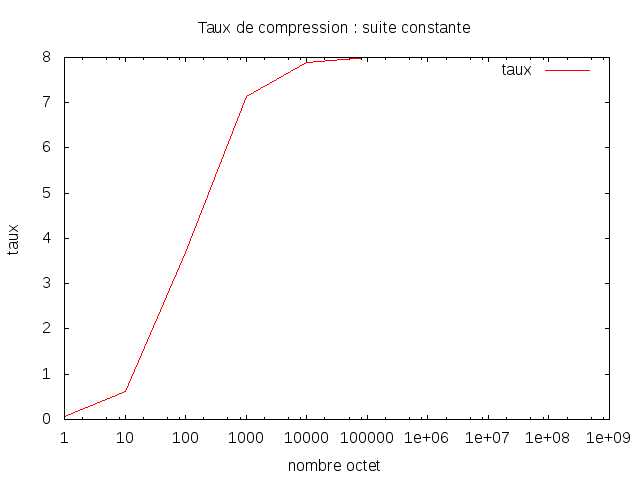
\includegraphics[width=7cm]{HConstant.png} & 
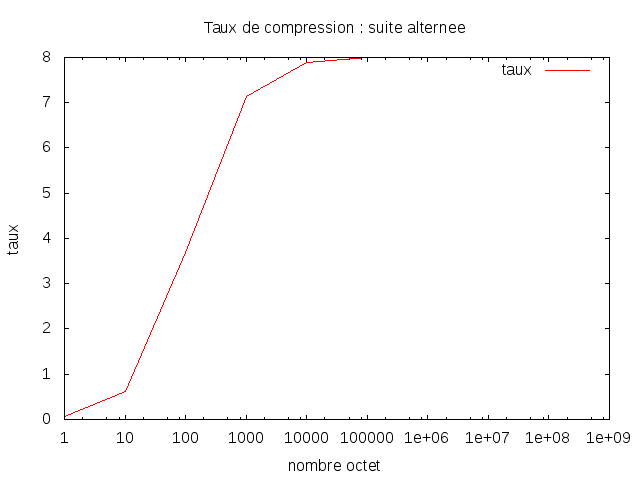
\includegraphics[width=7cm]{alternerH.png} 
\end{tabular}

\paragraph*{}
On peut voir ici que les  résultats de compression obtenue pour la suite constante et pour la suite alternée sont similaires, on observe des courbes constantes. En effet dans les deux cas, il n'y a qu'un seul caractère dans le fichier, soit le caractère codé par 00000000, soit le caractère codé par 10101010. Il y a donc un arbre à seulement 2 poids, la racine et la feuille et donc le caractère est codé sur un seul bit. On observe alors que le taux de compression tend rapidement vers 8 , car l'on remplace un octet par un bit. Ce n'est pas le cas sur des fichiers de plus faible taille car il faut compter le poids de l'arbre présent dans le fichier compresser.Ce poids, pour un arbre à une feuille étant de 13 octets.
\subparagraph*{}
\hspace{-2cm}\begin{tabular}{l | l}
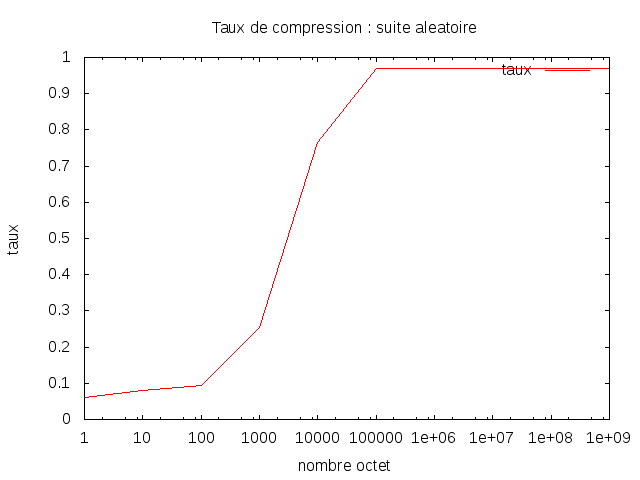
\includegraphics[width=7cm]{aleaH.png} & 
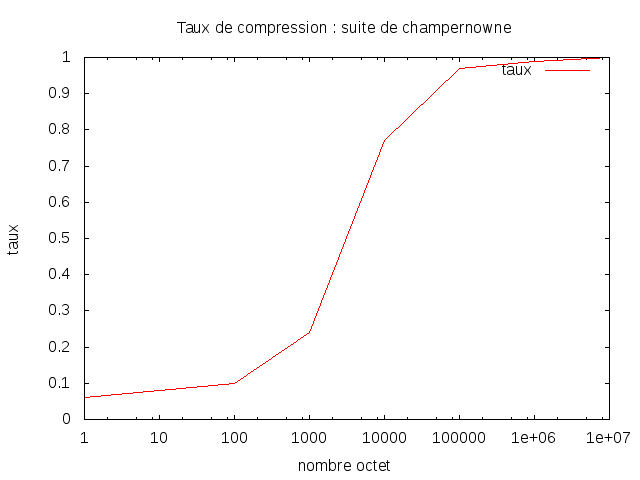
\includegraphics[width=7cm]{champH.png}
\end{tabular}
\paragraph*{}
Pour la suite aléatoire et la suite de Champernowne, le fichier ne compresse pas, au contraire il augmente. Cela viens du fait que les fréquences des multiples caractère sont à peu près équivalente. On ne peut donc pas réduire la taille des caractères. On remarque, que plus le fichier est petit, plus le taux de compression est faible (proche de 0). En cause le stockage l'arbre dans le fichier, qui est nécessairement plus grand que pour les suites constante ou alternée, étant donné qu'il n'y pas un caractère mais une multitude. Néanmoins, sur des fichiers de grande taille, le poids de l'arbre n'est pas significatif. 
Il y a cependant une différence entre la compression de la suite aléatoire et la suite de Champernowne. En effet, si la suite aléatoire n'atteint jamais vraiment son poids initial, du fait que chaque caractère à la même probabilité d'apparaître, le fichier compressé de la suite de Champernowne lui va revenir à son poids d'origine, car il fini par y avoir une répétition de certain motif du au caractéristique de la suite. \\ 

\newpage
\subsubsection{ Analyse de l'agorithme de Lemple Ziv}

Tout d'abord regardons nos fichiers composés que de 0, nous obtenons le graphique ci-dessous.
\begin{center}

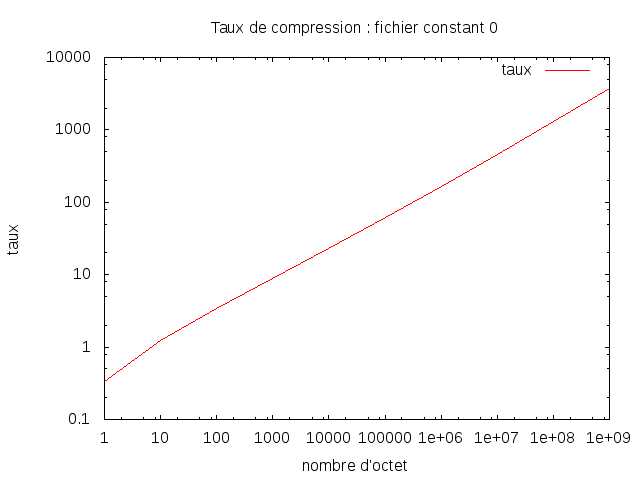
\includegraphics[width=10cm]{LZConstant.png}

\end{center}

On constate que la courbe est logarithmique, plus le nombre d'octet est important plus le taux de compression augmente. Ainsi le fichier compressé devient réellement de plus en plus petit. 
On remarque néanmoins que lorsque l'on veut compresser un seul octet le taux de compression est en dessous de 1, c'est-à-dire que le fichier compressé est plus gros que le fichier source. Ceci s'explique notamment par le stockage du premier  octet supplémentaire pour connaître le mode de compression, ici Lempel-Ziv. Il y a aussi une autre explication :  le début de compression pour Lempel-Ziv remplace un bit par 2 et ainsi de suite. Nous devons donc attendre les 10 octets dans le fichier source pour que la compression ai vraiment lieu. 
Lors de la compression d'un suite constante comme celle-ci, nous pouvons remarquer que l'arbre de compression est linéaire. En effet, il y a un seule branche composée de 0 les uns à la suite des autres. Le fait qu'il n'y ai qu'une seule branche explique en grande partie la performance de compression pour cette suite. 

\begin{center}
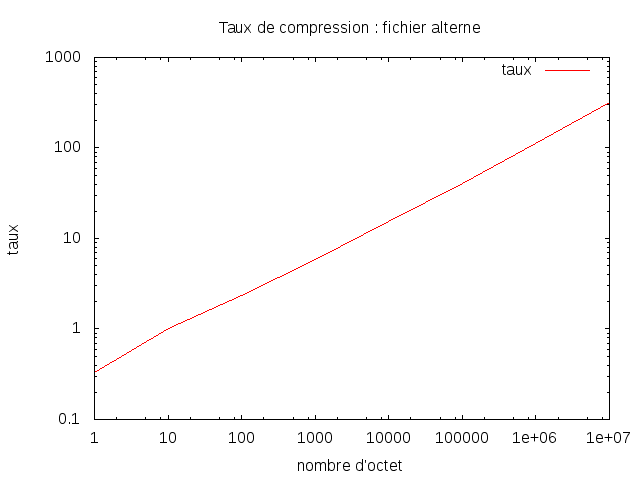
\includegraphics[width=10cm]{LZAlterner.png}
\end{center}

De même que sur le précédent graphique, la suite alternée a une compression dont le taux croît selon la taille de la suite. On constate que sur ce cas, l'arbre de compression quant à lui 2 branches au lieu d'une unique pour le cas constant. Ainsi on observe que la courbe du taux de compression augmente mais qu'elle n'est pas aussi efficace que pour le cas précédent, même si l'écart est plutôt faible.
Ici aussi, il faut attendre 10 octets pour que la compression débute, pour des raisons identiques à celle que nous avons déjà évoquées.  

\begin{center}
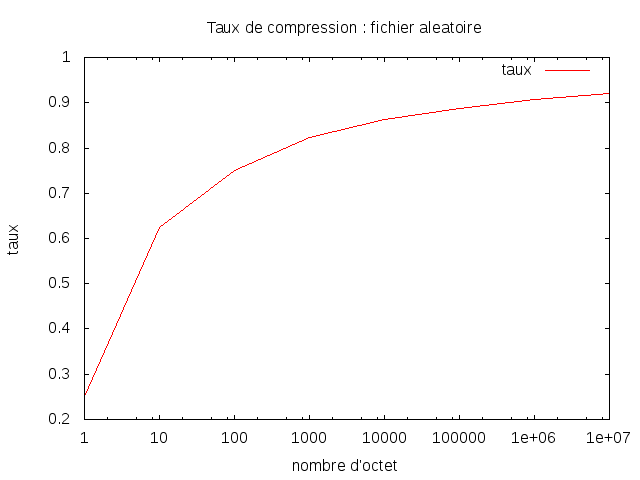
\includegraphics[width=10cm]{LZAleatoire.png}
\end{center}

On observe un changement avec les courbes précédentes, pour une suite aléatoire notre algorithme de compression n'a pas de bon résultat. En effet, le fichier obtenu à un nombre d'octet plus grand que le fichier source peu importe sa taille. Autrement dit, nous algorithme de compression ne compresse pas au contraire. 
On remarque néanmoins que plus le fichier source est grand, plus le taux de compression tend vers 1. Ceci s'explique notamment pas la taille de l'arbre de compression. Plus le fichier source est important, plus il y a de redondance dans les suites d'octets, ainsi on repasse obligatoirement par des chemins déjà existants, qui deviennent au fur et à mesure de plus en plus grand. 
C'est pour cela qu'on observe une courbe qui tend vers 1. 


\begin{center}
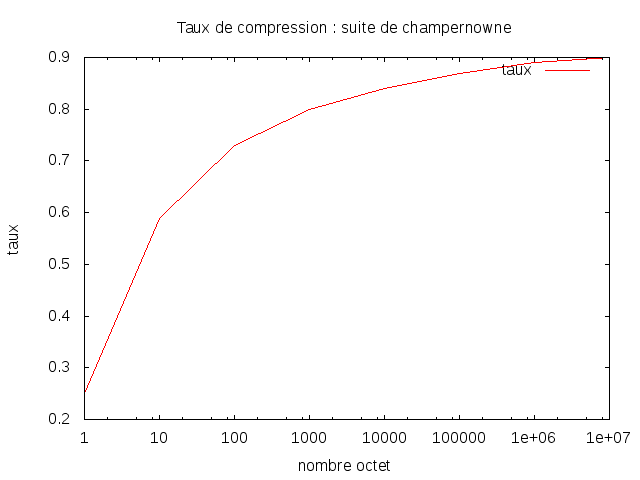
\includegraphics[width=10cm]{champLZ.png}
\end{center}
La suite de Champernowne est une suite très particulière pour notre algorithme. A chaque lecture nous allons créer dans notre arbre de compression un nouveau nœud dont la profondeur sera égal à la hauteur de l'arbre. Lorsque nous avancerons dans le processus, nous créerons tous les nœuds possible dans l'arbre ainsi comme la hauteur de l'arbre ne croîtra pas de façon logarithmique, nous n'aurons pas la possibilité d'avoir une compression satisfaisante. 
\newpage
\section*{Analyse du temps d’exécution}

\subsubsection*{Compression}
\paragraph*{}
\textbf{Temps d’exécution pour Huffman}
\subparagraph*{}
\hspace{-2cm}\begin{tabular}{l | l}
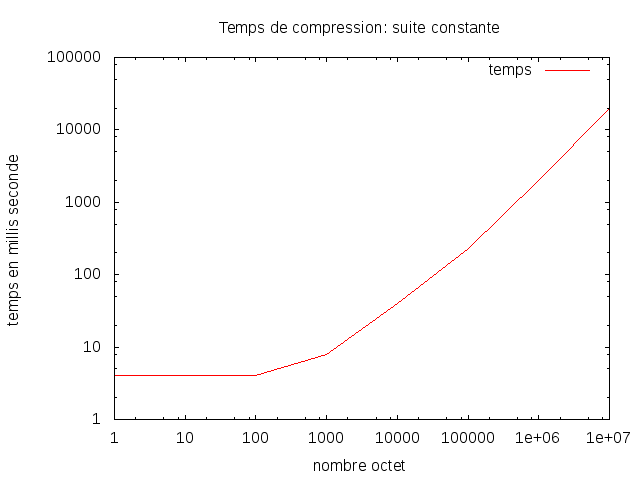
\includegraphics[width=7cm]{tempsChC.png} & 
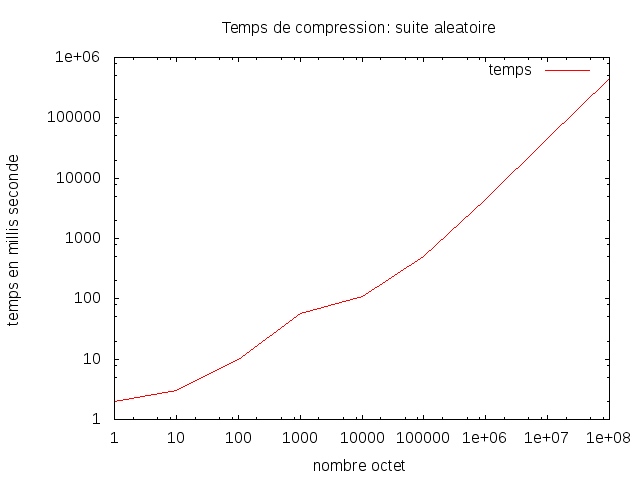
\includegraphics[width=7cm]{tempsChA.png}
\end{tabular}

\subparagraph*{}
Le temps d'exécution pour l'algorithme de Huffman est linéaire, plus le fichier source est important plus le temps d'exécution le devient. Cela est du à la lecture double du fichier source ainsi qu'à la construction de l'arbre. Lorsque le fichier source devient plus grand il faut lire beaucoup plus de caractère.    
On constate aussi, que la suite constante nécessite moins de temps pour être compressée que la suite aléatoire. Il y a 2 explications à cela. La première est le nombre de caractère à comparer. Pour la suite constante il n'y aucun caractère à comparer, contrairement à la suite aléatoire où nous devons comparer une multitude de caractères pour pouvoir les trier. La seconde explication découle de la première, en effet pour la suite constante l'arbre de compression ne possède que 2 poids et donc on le copie en un temps plus court qu'un arbre plus complexe comme celui de la suite aléatoire, qui est nécessairement plus grand.  

\newpage
\paragraph*{}
\textbf{Temps d’exécution pour Lempel-Ziv}
\subparagraph*{}
\hspace{-2cm}\begin{tabular}{l | l}
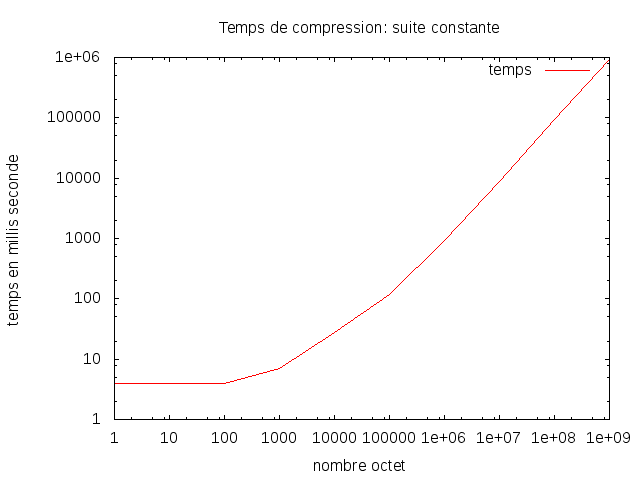
\includegraphics[width=7cm]{tempsClzC.png} & 
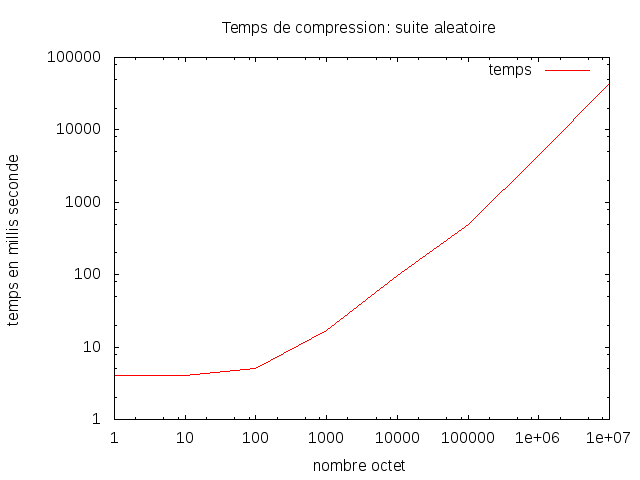
\includegraphics[width=7cm]{tempsClzA.png}
\end{tabular}

\subparagraph*{}
Le temps d'exécution pour l'algorithme de Lempel-Ziv est lui aussi linéaire. De la même façon le temps d'exécution croît en fonction du nombre d'octet présents dans le fichier source. Néanmoins, on remarque que pour la suite constante le temps d'exécution est plus rapide que pour la suite aléatoire. Ceci s'explique notamment par le parcours en profondeur de l'arbre. Dans le cas constant, plus le processus avance et plus le nombre d'octet lus est important avant la création d'un nœud dans l'arbre. De plus le nombre d'octet lu avant la création d'un nœud est logarithmique. Contrairement au cas constant, le cas aléatoire crée des nœuds dans l'arbre de façon plus fréquente. Il y a tout simplement moins de redondance dans le fichier source. Ainsi la création de ces multiples nœuds prend plus de temps, c'est donc une conséquence de la différence du temps d'exécution.

\paragraph*{}
En comparaison, les 2 algorithmes présentent des courbes pour le temps d'exécution linéaire. Néanmoins, l'algorithme de Lempel-Ziv a un temps d'exécution pour la compression plus rapide que pour celui de l'algorithme de Huffman. On l'observe de façon très significative dans la cas de la suite constante. Cette différence de rapidité est du à la lecture unique du fichier pour l'algorithme de Lempel-Ziv, contrairement à la lecture double du fichier pour l'algorithme de Huffman.	
\newpage
\paragraph*{}
\subsubsection*{Décompression}
\textbf{Temps d’exécution pour Huffman}
\subparagraph*{}
\hspace{-2cm}\begin{tabular}{l | l}
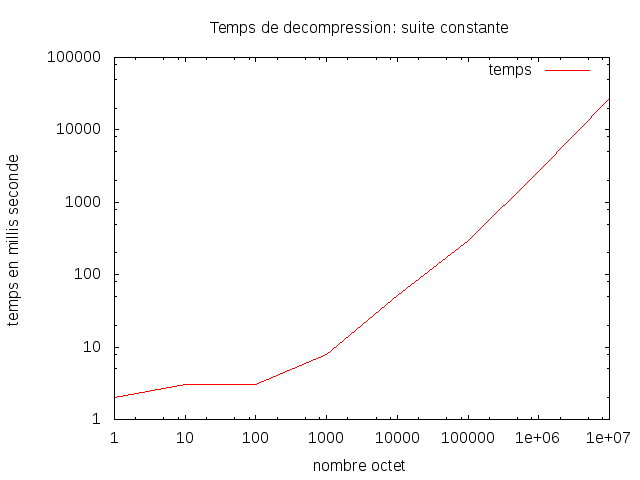
\includegraphics[width=7cm]{tempsDhC.png} & 
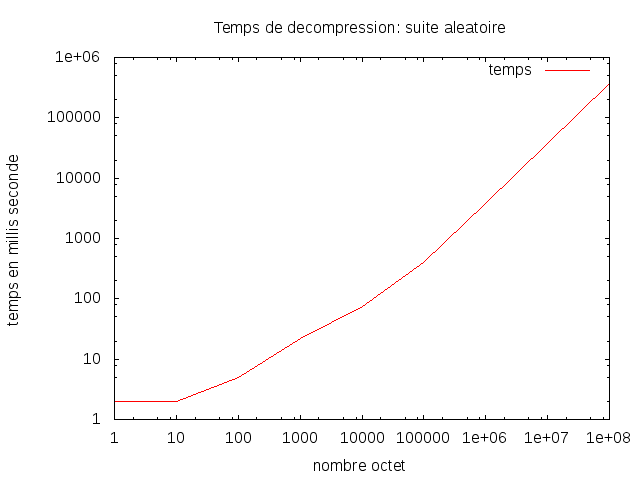
\includegraphics[width=7cm]{tempsDhA.png}
\end{tabular}
\subparagraph*{}
Le temps d'exécution pour la décompression de Huffman est linéaire. Ceci est notamment du à la lecture du fichier compressée, plus il est grand plus le nombre de caractère à traduire est important. 

Ce temps est très différent lorsqu’il s'agit d'une suite constante ou d'une suite aléatoire. Comme pour la compression il y a 2 explications à cela. La première est du à la lecture et au stockage en mémoire de l'arbre de compression, qui est plus grand pour la suite aléatoire. La seconde raison est, elle aussi liée à la lecture du fichier compressé. Comme il y a plus de caractère dans la suite aléatoire le code pour chaque lettre est donc plus grand, ainsi lors de la décompression il y a plus de caractère à lire dans le fichier compressé. Par conséquent, le temps de lecture de fichier est plus long.  

\newpage
\paragraph*{}
\textbf{Temps d’exécution pour Lempel-Ziv}
\subparagraph*{}
\hspace{-2cm}\begin{tabular}{l | l}
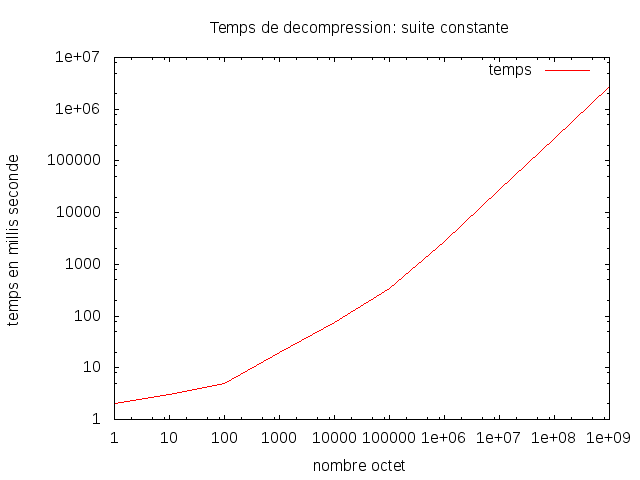
\includegraphics[width=7cm]{tempsDlzC.png} & 
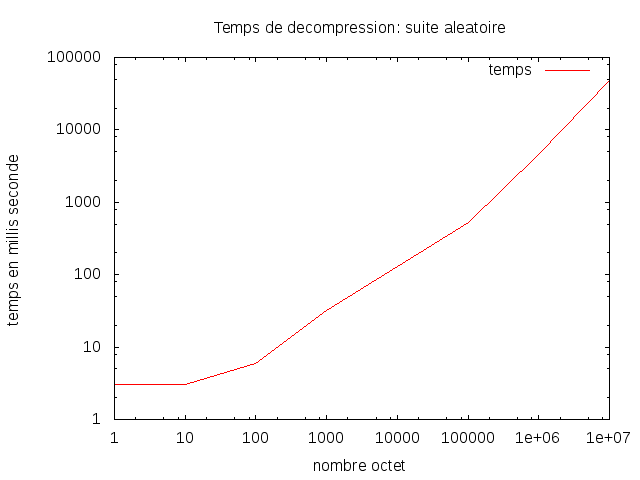
\includegraphics[width=7cm]{tempsDlzA.png}
\end{tabular}
\subparagraph*{}

Le temps d'exécution pour la décompression de Lempel-Ziv est lui aussi linéaire, pour les même raisons que celle évoquées précédemment.

De même, le temps pour décompresser une suite constante est plus faible que pour une suite aléatoire. De la même façon, cela s'explique par la taille du fichier compressé. En effet, le fichier compressé pour une suite constante a un poids très faible par rapport à un fichier compressé pour une suite aléatoire ayant le même nombre d'octet. Par conséquent, il est plus rapide de décompressée un fichier avec beaucoup de redondance.

\paragraph*{}
Le temps de décompression entre Huffman et Lempel-Ziv est très différent. Comme observé, Huffman est plus rapide que Lempel-Ziv. Cela est du à la création de l'arbre pour Lempel-Ziv qui a lieu en même temps que la lecture du fichier, ainsi il y a plus d'étape pour décompressé le fichier avec la méthode de Lempel-Ziv que celle de Huffman. Par conséquent Huffman est plus rapide à la décompression.

\newpage
\section*{Différences entre les algorithmes}
Dans cette dernière section, nous allons vous présenter un tableau avec plusieurs mode de compression et plusieurs type de fichiers. 
Nous expliquerons par la suite les différents taux de compression obtenus. 


\begin{flushleft}
{\renewcommand{\arraystretch}{2}
\begin{tabular}{|p{1.5cm}|p{1.5cm}|p{1.5cm}|p{1.5cm}|p{1.5cm}|p{1.5cm}|p{1.5cm}|p{1.5cm}|}
\hline
 & La bible (en anglais)  & Les Fleurs du Mal  & Au bonheurs des Dames & fichier PDF & musique  MP3 & image JPG & vidéo MOV\\
\hline
taille réélle (en octet)  & 883 158 & 180 199 & 952 753 & 198 931 & 8 843 546 & 3 988 442 & 54301053 \\\hline
zip & 3,44 & 2,51 & 2,57 & 1,246 & 1,065 & 1,002 & 1,0003 \\
\hline
Gzip & 3,44 & 2,51 & 2,644 & 1,247 & 1,065 & 1,002 & 1,0001 \\
\hline
Bzip2 & 4,89 & 3,045 & 3,719 & 1,212 & 1,063 & 1,005 & 0,9961\\
\hline
XZ & 4,649 & 2,826 & 3,323 & 1,261 & 1,066 & 1,002 & 1,0004\\
\hline
Huffman & 1,725 & 1,688 & 1,747 & 0,998 & 1,021 & 0,999 & 0,9999 \\
\hline
Lempel-Ziv & 1,796 & 1,310 & 1,482 & 0,933 & 0,979 & 0,929 & 0,9269\\
\hline

\end{tabular}
}
\end{flushleft}

Tout d'abord, nous observons que les différents compresseurs sur le marché fonctionnent de façon bien plus efficace que nos compresseurs. Ceci-ci s'explique car ces processus allient plusieurs algorithmes qu'ils appliquent les uns après les autres. Zip et Gzip utilisent un algorithme de Deflate qui couple le codage d'un algorithme de Lempel-Ziv plus complexe (LZ77) et le codage de Huffman. Bzip2 , utilise  la transformée de Burrows-Wheeler (méthode de réorganisation des données) avec le codage de Huffman. Enfin XZ utilise l'algorithme de LZMA , c'est à dire Lempel-Ziv-Markov-chain Algorithm, c'est un algorithme qui associe Lemepel-Ziv et les chaînes de Markov.

Nous avons choisit ces 4 modèles de comparaison car ce sont tous des algorithmes de compression sans perte. 

Regardons les résultats des romans. Comme on peut le constater, nous avons décidé de faire des tests sur la Bible qui est en anglais, mais aussi sur un fichiers de même taille en français "Aux bonheurs des Dames" et sur un livre de plus petite taille, en français  : "Les Fleurs du Mal". Tout d'abord commençons par les 2 livres en français. On constate que tous les compresseurs obtiennent un meilleur taux avec "Aux bonheurs des Dames" car il est tous simplement plus gros donc avec forcément plus de redondance. De plus Huffman à un meilleur taux que Lempel-Ziv ce qui est du à la grande redondance de la langue française. 
 Au contraire, pour la Bible, c'est Lempel-Ziv qui à un meilleur taux de compression que Huffman. Ceci est du à la plus faible redondance de lettre dans la langue anglaise et à la forte répétition de mot qui rend Lempel-Ziv plus efficace.
Voilà pourquoi aussi tous les compresseurs ont un meilleurs taux avec la Bible qu'avec "Aux bonheurs des Dames" , ils utilisent un modèle qui ne repose pas que sur la redondance des lettres. 

Regardons maintenant les 4 dernières colonnes. Elles ont toutes les 4 un point commun : leurs extensions de fichier sont déjà des mode de compression. En effet, MP3 est un mode de compression avec perte, MOV est un mode de compression de vidéo développé par Apple , PDF est un format favorisant la portabilité des documents par la compression de celui -ci, et JPG ou JPEG est une compression d'image matricielle. Ainsi comme nous le constatons aucun des compresseurs n'a de bon taux. Pour les compresseurs sur le marché, il garde à peu près le même nombre d'octet que le fichier source. Pour nos compresseurs, le taux est plus faible et dans la plupart des cas il n'y a pas de compression. 

Nous pouvons donc remarquer que les compresseurs sur le marché ont un bien meilleur rendement que les nôtres.



\section*{Conclusion}
Au cours de ce projet, nous avons pu implémenter deux algorithmes de compression :  Huffman statique et Lempel-Ziv. Ceci nous à permis de découvrir un codage entropique : Huffman. Comme observé,le codage entropique nécessite le stockage de l'arbre de compression et une double lecture du fichier source. Par conséquent, on obtient de temps de décompression plus rapide malgré un fichier compressé alourdi par le stockage de l'arbre. De plus, l'algorithme de Huffman,s'appuyant sur la redondance de caractère,ne peut dépassez un taux de compression supérieur à 8.

Nous avons aussi découvert un codage algorithmique : Lempel-Ziv. Celui-ci n'a pas à transmettre d'information pour la décompression, mais nécessite une reconstruction de l'arbre lors de la décompression. Ainsi le taux de compression est meilleur malgré un temps d'exécution pour la décompression plus important.L'algorithme de Lempel-Ziv s'appuyant sur la répétition de motif , son taux de compression ne connait pas de limite.

Par ailleurs, nous avons constaté, que les compresseurs sur le marché ont un meilleurs taux de compression tout type de fichier confondu. Ces compresseurs utilisent des alliances entre différents algorithmes de compression et différents codages. De plus, des nouveaux compresseurs arrivent encore, comme la découverte de Olivier Thomine qui a crée un compresseur qui permet de compresser des données environs 10 000 fois plus rapidement d'un algorithme de Lempel-Ziv-Welch. \footnote{http://www.futura-sciences.com/magazines/high-tech/infos/actu}.La compression de fichier est un domaine de recherche important en informatique.


\end{document}